% vim: set textwidth=78 autoindent:

\subsection{Quick Print Plugin}

% when the revision of a section has been finalized, 
% comment out the following line:
% \updatedisclaimer

The \toolbtntwo{quick_print}{Quick Print} Plugin allows to print the current 
map canvas with minimal effort into PDF format. All the user needs to add 
is a Map Title, a Map Name and the Paper Size (See Figure~\ref{fig:quickprint}). 
\begin{figure}[ht]
   \begin{center}
   \caption{Quick Print Dialog \nixcaption}\label{fig:quickprint}\smallskip
   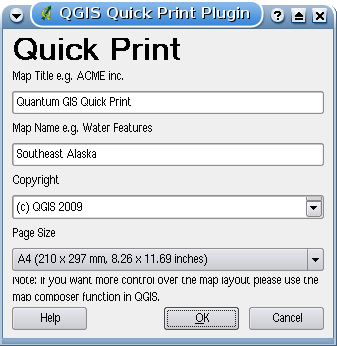
\includegraphics[clip=true, width=6cm]{quick_print_dialog}
\end{center}
\end{figure}

Figure~\ref{fig:quickprint_result} below shows a DIN A4 quick print result 
from the alaska sample dataset. If you want more control over the map layout, 
please use the print composer plugin, described in 
Section~\ref{label_printcomposer}.  

\begin{figure}[ht]
   \begin{center}
   \caption{Quick Print result as DIN A4 PDF\nixcaption}\label{fig:quickprint_result}\smallskip
   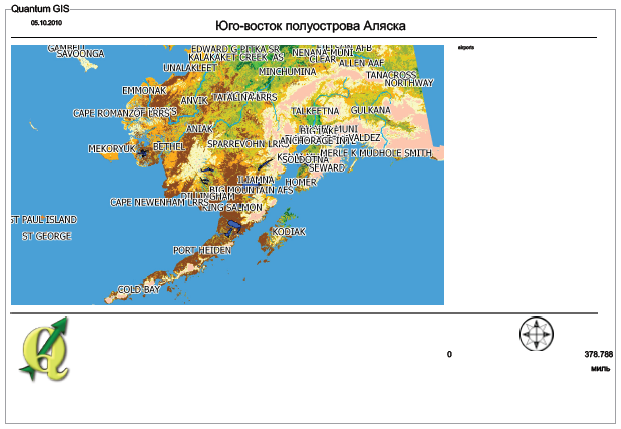
\includegraphics[clip=true, width=11cm]{quick_print_result}
\end{center}
\end{figure}


